\documentclass[]{article}
\usepackage{lmodern}
\usepackage{amssymb,amsmath}
\usepackage{ifxetex,ifluatex}
\usepackage{fixltx2e} % provides \textsubscript
\ifnum 0\ifxetex 1\fi\ifluatex 1\fi=0 % if pdftex
  \usepackage[T1]{fontenc}
  \usepackage[utf8]{inputenc}
\else % if luatex or xelatex
  \ifxetex
    \usepackage{mathspec}
  \else
    \usepackage{fontspec}
  \fi
  \defaultfontfeatures{Ligatures=TeX,Scale=MatchLowercase}
\fi
% use upquote if available, for straight quotes in verbatim environments
\IfFileExists{upquote.sty}{\usepackage{upquote}}{}
% use microtype if available
\IfFileExists{microtype.sty}{%
\usepackage{microtype}
\UseMicrotypeSet[protrusion]{basicmath} % disable protrusion for tt fonts
}{}
\usepackage[margin=1in]{geometry}
\usepackage{hyperref}
\hypersetup{unicode=true,
            pdfborder={0 0 0},
            breaklinks=true}
\urlstyle{same}  % don't use monospace font for urls
\usepackage{graphicx,grffile}
\makeatletter
\def\maxwidth{\ifdim\Gin@nat@width>\linewidth\linewidth\else\Gin@nat@width\fi}
\def\maxheight{\ifdim\Gin@nat@height>\textheight\textheight\else\Gin@nat@height\fi}
\makeatother
% Scale images if necessary, so that they will not overflow the page
% margins by default, and it is still possible to overwrite the defaults
% using explicit options in \includegraphics[width, height, ...]{}
\setkeys{Gin}{width=\maxwidth,height=\maxheight,keepaspectratio}
\IfFileExists{parskip.sty}{%
\usepackage{parskip}
}{% else
\setlength{\parindent}{0pt}
\setlength{\parskip}{6pt plus 2pt minus 1pt}
}
\setlength{\emergencystretch}{3em}  % prevent overfull lines
\providecommand{\tightlist}{%
  \setlength{\itemsep}{0pt}\setlength{\parskip}{0pt}}
\setcounter{secnumdepth}{0}
% Redefines (sub)paragraphs to behave more like sections
\ifx\paragraph\undefined\else
\let\oldparagraph\paragraph
\renewcommand{\paragraph}[1]{\oldparagraph{#1}\mbox{}}
\fi
\ifx\subparagraph\undefined\else
\let\oldsubparagraph\subparagraph
\renewcommand{\subparagraph}[1]{\oldsubparagraph{#1}\mbox{}}
\fi

%%% Use protect on footnotes to avoid problems with footnotes in titles
\let\rmarkdownfootnote\footnote%
\def\footnote{\protect\rmarkdownfootnote}

%%% Change title format to be more compact
\usepackage{titling}

% Create subtitle command for use in maketitle
\newcommand{\subtitle}[1]{
  \posttitle{
    \begin{center}\large#1\end{center}
    }
}

\setlength{\droptitle}{-2em}
  \title{}
  \pretitle{\vspace{\droptitle}}
  \posttitle{}
  \author{}
  \preauthor{}\postauthor{}
  \date{}
  \predate{}\postdate{}

\usepackage{graphicx,latexsym}
\usepackage{amssymb,amsthm,amsmath}
\usepackage{longtable,booktabs,setspace}

\begin{document}

\section{Desarrollo de Orthocore e implementación de otras herramientas
computacionales para entender el pangenoma de un linaje
genómico.}\label{desarrollo-de-orthocore-e-implementacion-de-otras-herramientas-computacionales-para-entender-el-pangenoma-de-un-linaje-genomico.}

\begin{figure}[h!tbp]
\centering
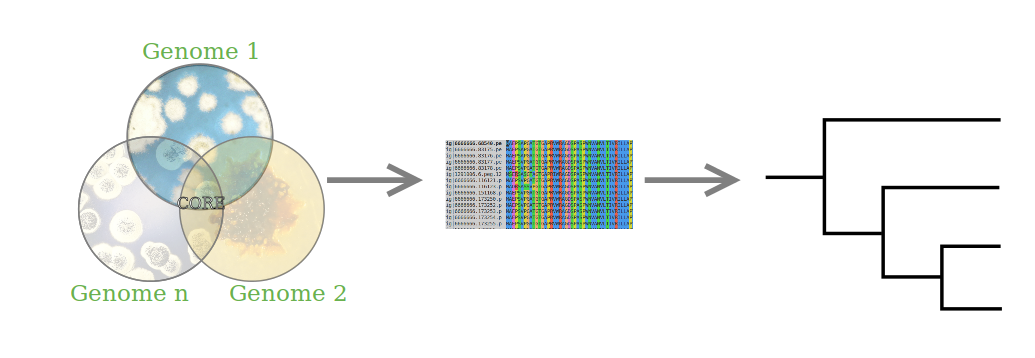
\includegraphics[angle = 0,scale = .42]{chapter1/coreWiki.png}
\caption[Orthocore calcula el core de un linaje genómico para proveer una filogenia]{\footnotesize{Orthocore calcula las familias génicas comunes de un linaje genómico. Después de un proceso de filtrado, alineamiento y curación concatena estas familias y entrega una reconstrucción filogenética.}}
\label{fig:Orthocore}
\end{figure}

El pangenoma es el contenido génico total de un linaje taxonómico. Las
familias génicas de un pangenoma pueden clasificarse según sus patrones
de presencia-ausencia en cada genoma del linaje. De acuerdo a esta
clasificación los principales grupos de familias génicas en un pangenoma
son el \emph{core}, el \emph{shell} y el \emph{cloud} (dispensable)
genome. El \emph{core genome} es el conjunto de familias con presencia
en todos los genomas del linaje. Por ejemplo, la secuencia de la
subunidad 16s del gene rRNA, así como diversos genes ribosomales que
suelen estar en el core de la gran mayoría de los linajes bacterianos.
El \emph{shell genome} es el grupo de familias presentes en la mayoría
de los genomas pero no en todos. En el \emph{shell} se ubican por
ejemplo familias que estaban en el \emph{core genome} pero que algunas
bacterias del linaje sufrieron una dinámica de pérdida (o ganancia)
génica. Mientras que el \emph{cloud genome} o dispensable genome es
aquel grupo de familias que sólo ocurre en unos cuantos genomas del
linaje.

La organización filogenética de un linaje genómico permite la
observación de pérdida y ganancia de familias génicas en organismos
cercanos. Si los organismos están desordenados es difícil apreciar la
dinámica genómica de aparición-desaparición de miembros de una familia
génica. Ordenar los genomas de un linaje facilita apreciar cambios en el
número de copias de una familia. Esto es relevante en el marco de esta
tesis ya que cambios en los perfiles de promiscuidad podrían estar
relacionados a copias extras de organismos cercanos. Orthocore es un
algoritmo que utiliza el core conservado de un linaje genómico para
facilitar la organización filogenética de sus organismos
\autoref{fig:Orthocore}

\subsection{La distribución de la función metabólica de las familias del
pangenoma depende de la variabilidad del linaje
seleccionado.}\label{la-distribucion-de-la-funcion-metabolica-de-las-familias-del-pangenoma-depende-de-la-variabilidad-del-linaje-seleccionado.}

El número de familias génicas presentes en el pangenoma, así como su
distribución en el \emph{core}, \emph{shell} y \emph{dispensable genome}
depende de la elección de los genomas y del linaje genómico. Para
entender esto se puede pensar en un ejemplo extremo, consideremos una
bacteria de 1000 familias de genes de la cual se obtienen secuencias de
diez genomas de la misma cepa. Estas secuenciaciones deberían ser
prácticamente idénticas y en ese caso el \emph{core genome} sería 1000
familias, el \emph{shell} y el \emph{dispensable genome} serían cero. En
este caso, todo el metabolismo, tanto el central como el especializado
estarían conservados dentro del \emph{core genome}, ya que el
\emph{shell} y el \emph{dispensable genome} se encuentran vacíos. Sin
embargo, si variamos el linaje taxonómico, y ahora estudiamos el
pangenoma de 10 especies distintas del género \emph{Streptomyces} ahora
el core genome estará compuesto por aproximadamente un tercio de su
tamaño promedio, y dentro del \emph{core genome} es donde se encontrarán
muchos de las familias dedicadas al metabolismo central o conservado
(por ejemplo, familias de la glicólisis o síntesis de aminoácidos). En
cambio muchas de las familias dedicadas al metabolismo especializado y
pertenecientes a clústers biosintéticos de productos naturales (BGCs)
estarán en el \emph{dispensable genome} pues \emph{Streptomyces} es
productor de una gran variedad de metabolitos especializados y cada
especie suele tener su producto característico.
\autoref{fig:MetabolismoPangenoma}

\begin{figure}[h!tbp]
\centering
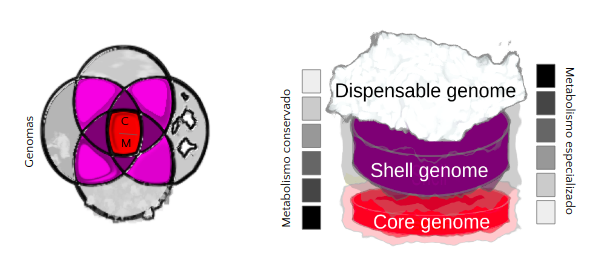
\includegraphics[angle = 0,scale = .75]{chapter1/Metabolismo-Pangenoma.png}
\caption[El metabolismo en el Pangenoma]{\footnotesize{El pangenoma de un conjunto de genomas de un linaje puede ser clasificado en varios grupos. En este ejemplo, en el lado izquierdo de la figura se observa en gris el $genoma~dispensable$ compuesto por familias génicas presentes sólo en un genoma. En dos tonos de morado observamos el $shell genome$, familias que están presentes en la mayoría de los genomas del linaje, en este en caso dos o tres genomas. Finalmente en rojo se muestra el $core$, aquellas familias presentes en todos los genomas del linaje. El $core$ contiene tanto familias muy conservadas con una sola copia por genoma ( C ), como familias expandidas. Las familias marcadoras (M) pueden ser parte del $core$ conservado o de las familias expandidas. Del lado derecho se muestra una representación del pangenoma para cualquier número de genomas. Familias de metabolismo conservado tenderán a estar concentradas entre el $core$ y el $shell~genome$, mientras que el metabolismo especializado tendrá más representantes en el dispensable que en el $core genome$. Sin embargo tanto el tipo de metabolismo como el tamaño del $core$, $shell$ y $genoma~dispensable$ pueden variar según la diversidad de los organismos seleccionados. }}
\label{fig:MetabolismoPangenoma}
\end{figure}

El \emph{core genome} de un linaje, además de tener familias conservadas
y prácticamente presentes en todo el dominio Bacteria también puede
contener familias marcadoras \autoref{fig:CoreMarcadores} . Estos genes
marcadores permiten realizar pruebas de diagnóstico para colonizaciones
bacterianas. A las familias que están presentes en el \emph{core genome}
de un linaje A, pero que están completamente ausentes de un linaje B se
les llama marcadoras. Por ejemplo genes conservados en la especie
\emph{Streptomyces coelicolor} pero no conservados en \emph{Streptomyces
rimosus} son genes marcadores de \emph{Streptomyces coelicolor} respecto
de \emph{Streptomyces rimosus}. Estos mismos marcadores tal vez no sean
marcadores respecto de \emph{Streptomyces lividans}, a pesar de la
cercanía taxonómica entre estos organismos. La presencia de genes
marcadores en el core depende de ambos linajes, por lo que es importante
contar con algoritmos que permitan automatizar su cálculo.

El número de familias en el pangenoma, ya sea en el \emph{core, shell o
dispensable} genome no sólo depende de la divergencia o proximidad
taxonómica de los organismos del linaje seleccionado, también depende de
lo variable que sea el contenido génico en los genomas del linaje. A
esta característica se le conoce como apertura. Hay especies, por
ejemplo algunos patógenos, cuyo pangenoma se encuentra sumamente cerrado
en el sentido de que no importa cuántos genomas se agreguen, el número
de familias parece converger y ser asintótico rápidamente a una cota
superior. En cambio especies o géneros que viven en una gran diversidad
de hábitats suelen tener un pangenoma abierto. Esto significa que cada
vez que se agrega un nuevo genoma aparecen otras familias que no estaban
en los genomas anteriores. En los linajes con pangenoma abierto el
número de familias nuevas al agregar un genomas seguirá una tendencia
creciente y no asintótica.

Además de la apertura, existen otros intentos de cuantificar la
diversidad génica de un linaje. Está por ejemplo la fluidez, definida
como el promedio de familias únicas entre familias totales por pares de
genomas. El pangenoma bacteriano total, es decir el total de familias
génicas en el dominio Bacteria es considerado abierto.

\begin{figure}[h!tbp]
\centering
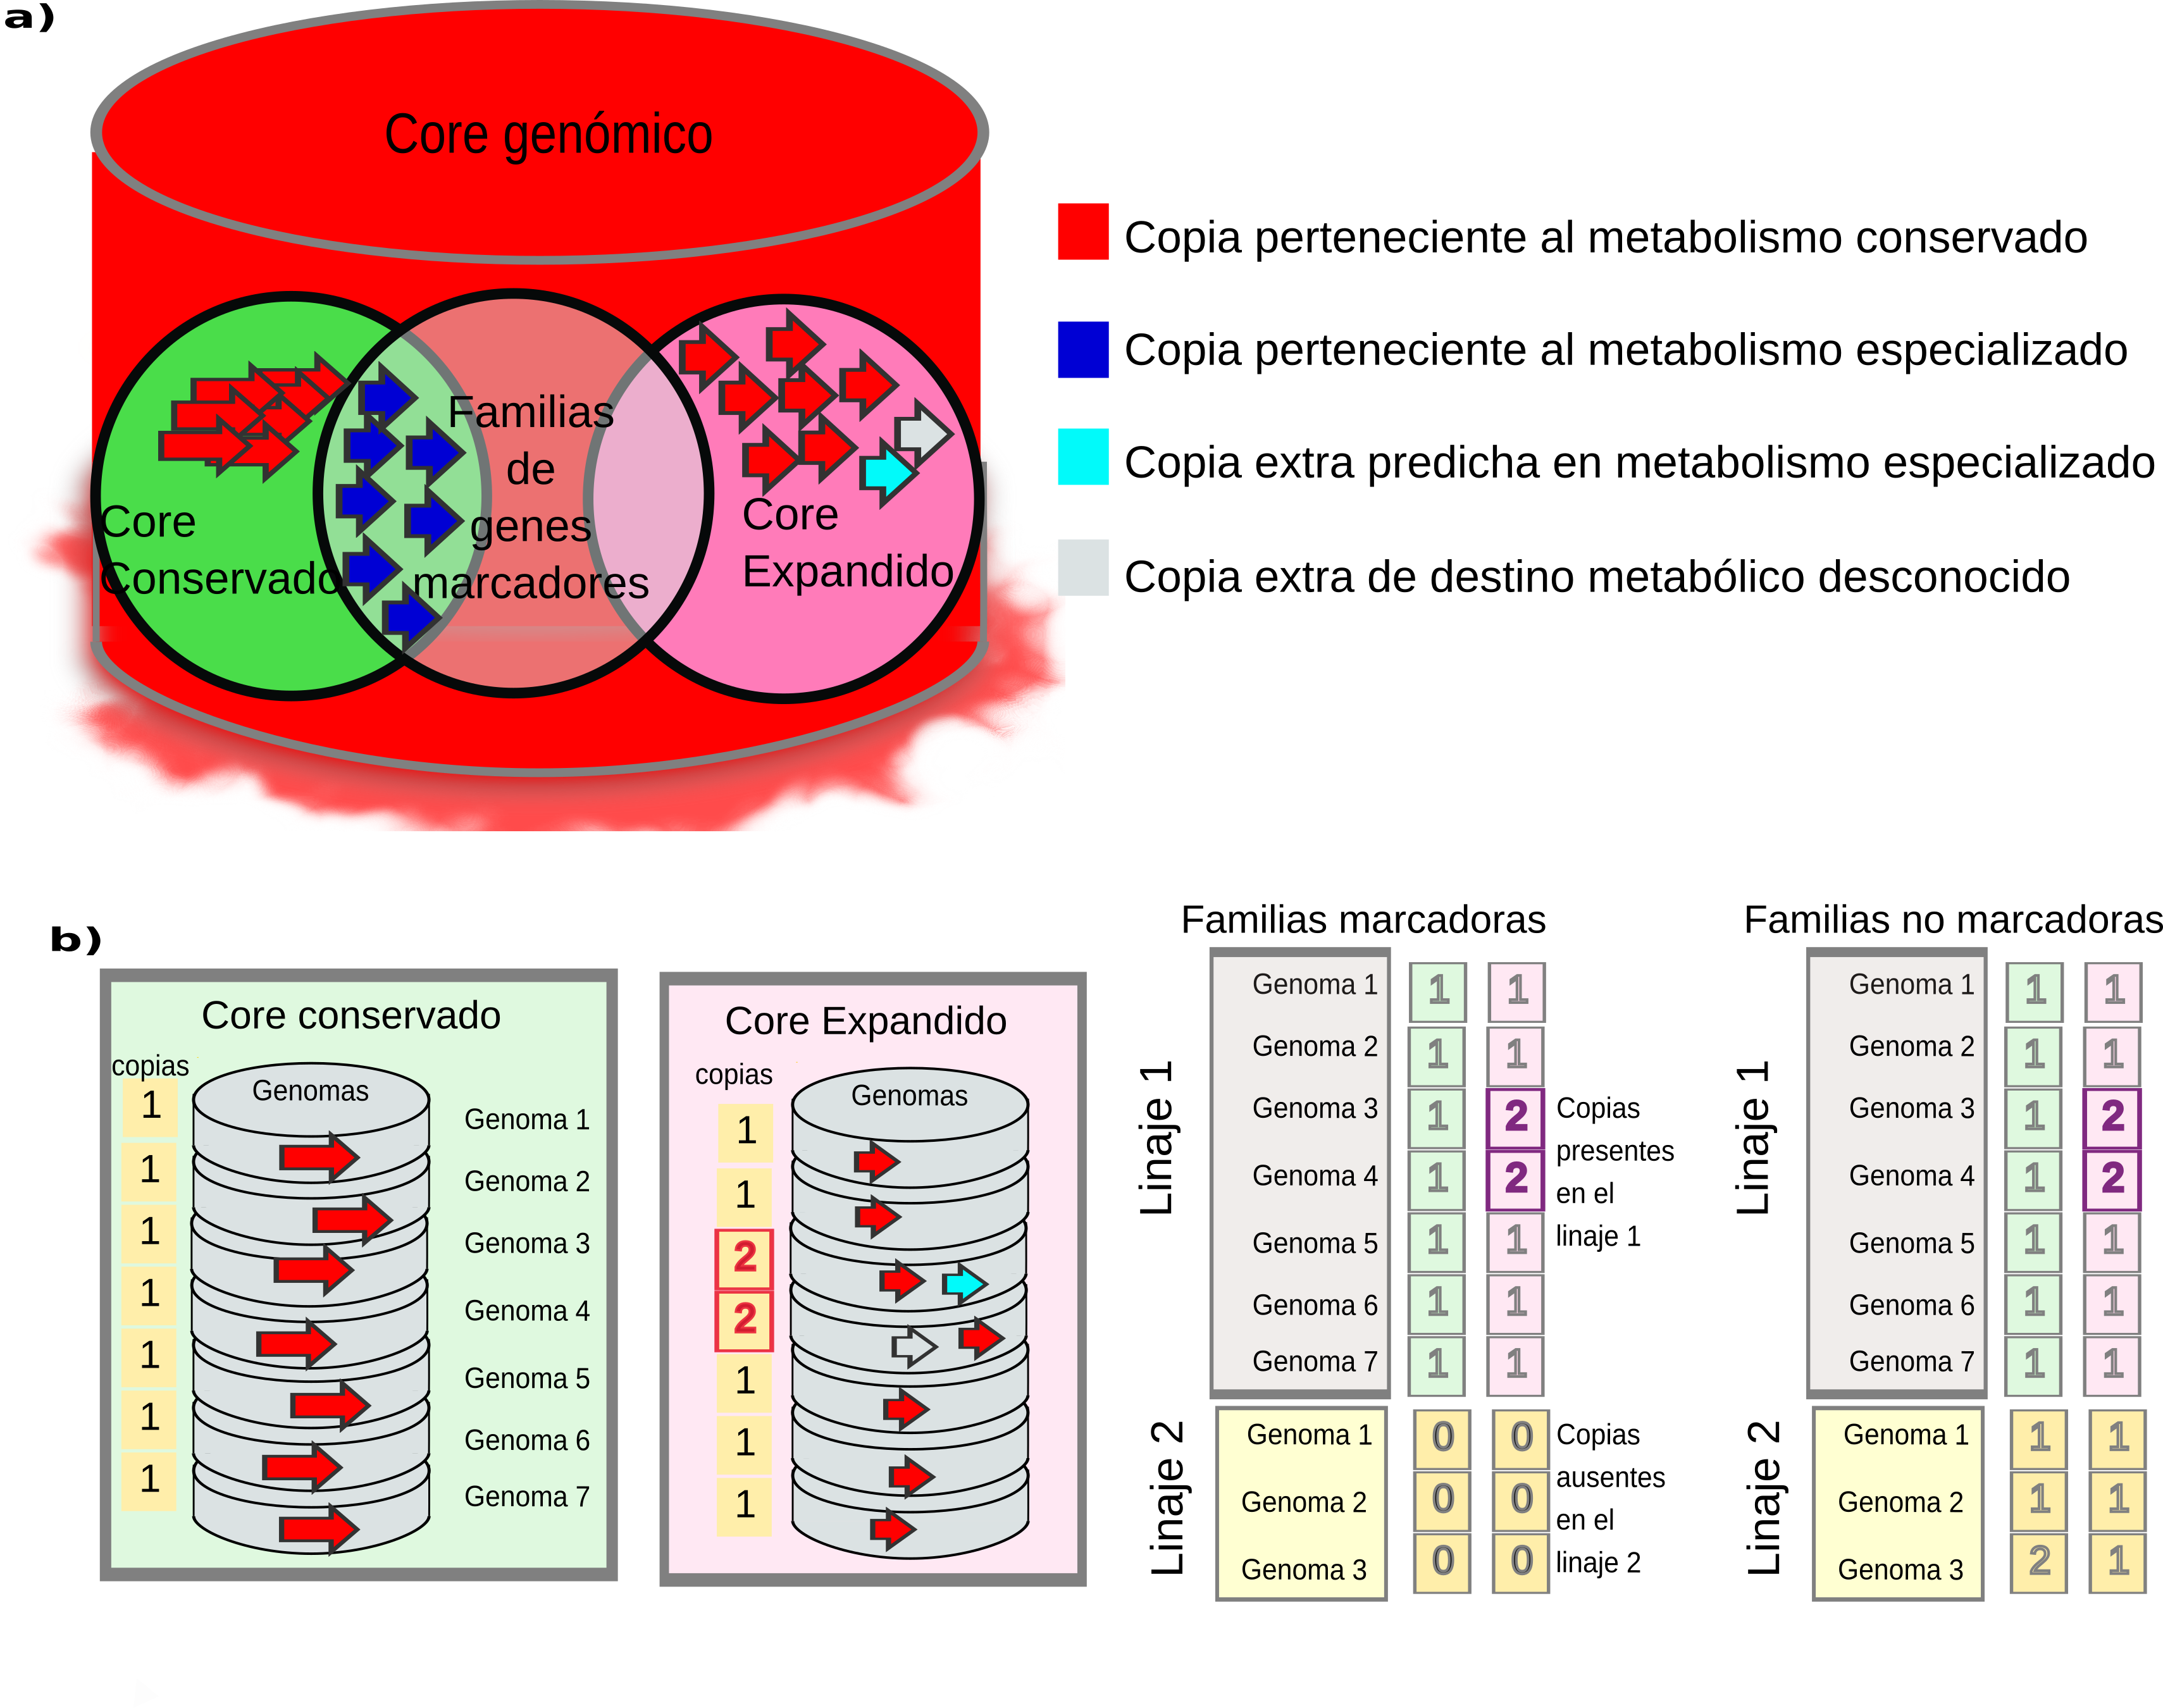
\includegraphics[angle = 0,scale = .8]{chapter1/CoreMarcadores.png}
\caption[Core y genes Marcadores]{\footnotesize{El core genome puede contener familias con funciones en distintos grupos metabólicos así como diversidad en el número de copias. Arriba se muestra que en el core pueden coexistir familias tanto de copia única como con expansiones. Las familias con funciones en el metabolismo conservado suelen concentrarse en el $core~genome$ (rojas), pero también dependiendo de los organismos seleccionados pueden encontrarse ya sea familias enteras o algunas copias dedicadas al metabolismo especializado (azul). No de todas las copias se conocerá su función, algunas pueden tener un destino metabólico desconocido (gris) o bien ser predichas por algún algoritmo como parte del metabolismo especializado (cyan).  Abajo a la izquierda se comparan familias del $core~conservado$ con exactamente una copia por genoma contra familias del $core~expandido$. Ambas pertenecen al $core$, pero en el $core~expandido$ hay dos genomas que tienen una copia extra en esta familia, unoa cyan y una gris, que podría dificultar la elección de los verdaderos ortólogos. A la derecha se ejemplifican familias de genes marcadores, útiles para identificar un linaje genómico. Tanto familias del $core~conservado$ como del $core~expandido$ pueden ser familias marcadores, siempre que exista al menos una copia de cada familia en el linaje 1 y ninguna copia en el linaje 2. Las familias dejan de ser marcadoras cuando el linaje dos contiene al menos una copia en algún genoma.}}
\label{fig:CoreMarcadores}
\end{figure}

Finalmente la distribución de las funciones metabólicas encontrada en
los subconjuntos del pangenoma ( \emph{core, shell y dispensable}
genome) está relacionada a la proximidad filogenética de los organismos
seleccionados en el estudio. Entre más diversos sean los organismos
menos familias dedicadas exclusivamente a metabolismo especializado
abundarán en el \emph{core/shell genome}. La diversidad provocará que lo
único que tengan los genomas de estos organismos en común sean funciones
conservadas por una amplia variedad de especies bacterianas. Ahora bien,
muchas familias de metabolismo especializado provienen de reclutamientos
de copias extra de familias de metabolismo conservado. Así pues aunque
decrezca el número de familias con exclusividad en metabolismo
especializado en el \emph{core y shell genome}, estos sunconjuntos del
pangenoma aún pueden contener familias conservadas que tengan copias
extra en proceso de reclutamiento para algún Cluster biosintético de
genes (BGCs) de metabolismo especializado. Considerando las reflexiones
anteriores, entre más diverso sea un linaje, más tenderá su \emph{core
genome} a contener exclusivamente familias de metabolismo conservado
mientras que su dispensable genome estará formado mayormente por
familias de enzimas del metabolismo especializado.

\subsection{El core conservado permite la reconstrucción de filogenias
complicadas}\label{el-core-conservado-permite-la-reconstruccion-de-filogenias-complicadas}

Orthocore es el desarrollo bioinformático que realicé para calcular las
familias génicas más conservadas del \emph{core genome}. Dos genes son
homólogos si poseen un ancestro común, entre los principales grupos de
homólogos están ortólogos y parálogos. Los ortólogos provienen de
eventos de especiación de un ancestro común mientras que los parálogos
evolucionan por eventos de duplicación. Orthocore obtiene un subconjunto
del \emph{core genome}: el \emph{core conservado}, es decir, familias de
ortólogos presentes en todos los genomas del grupo y que además son
libres de parálogos de difícil identificación. El \emph{core conservado}
facilita la organización en árboles filogenéticos de organismos de un
linaje genómico.

La comparación de la variación molecular entre ortólogos ha sido
utilizada para establecer relaciones filogenéticas entre organismos.
Esta técnica ha dado lugar a grandes descubrimientos. Por ejemplo
comparar la secuencia de la subunidad 16s del gene RNA ribosomal condujo
a Woese al descubrimiento del dominio Archaea en 1977
{[}@woese\_phylogenetic\_1977{]}. Un árbol de especies suele hacerse con
secuencias de familias que pertenecen al core genome de un Dominio, por
ejemplo las familias 16s o RpoB en los Dominios Bacteria y Archaea.
Algunos autores realizan árboles multilocus para mejorar la resolución
de árboles de especies realizados mediante la comparación de secuencias
de 16s. Los genes seleccionados para los árboles multilocus deben estar
en todos los organismos y no tener copias extra tan parecidas que puedan
confundirse y entorpecer la reconstrucción filogenética, es decir, las
familias seleccionadas deben ser parte del \emph{core conservado}.
Orthocore automatiza la identificación de estas familias.

Entre los factores importantes para establecer las relaciones
filogenéticas diferenciando entre Archaea y Bacteria están los
siguientes: 1) la presencia conservada de la subunidad de 16s en los
tres dominios mencionados, y 2) la suficiente divergencia entre estas
secuencias en los organismos de dichos dominios. Ahora bien, establecer
relaciones filogenéticas entre Archaea y Bacteria es en cierto sentido
más sencillo que establecerlas entre organismos pertenecientes al mismo
género o inclusive a la misma especie. En ocasiones, como en el caso del
género \emph{Streptomyces}, la secuencia de 16s por sí sola no posee la
suficiente variación para resolver la filogenia
{[}@labeda\_phylogenetic\_2017{]}. En \emph{Streptomyces} la variación
entre estas secuencias suele ser menor al 1\%. Para resolver el problema
de escasa variación en secuencias de 16s se pueden concatenar las
secuencias de otros ortólogos, siempre que estos aparezcan en todos los
organismos que se estén estudiando, es decir, siempre que sean parte del
core genómico.

\subsection{El algoritmo de Orthocore}\label{el-algoritmo-de-orthocore}

\begin{figure}[h!tbp]
\centering
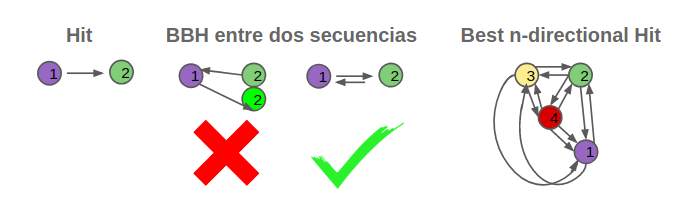
\includegraphics[angle = 0,scale = .55]{chapter1/Best-n-directional.png}
\caption[Los mejores hits n-direccionales generalizan a los $Bidirectional~Best~Hits$]{\footnotesize{Orthocore utiliza los mejores hits n-direccionales para obtener grupos de ortólogos. Un hit es el mejor resultado de una secuencia en otro genoma. Un Bidireccional Best Hit es el mejor hit bidireccional. La secuencia 2 es el mejor hit de la secuencia 1 en el genoma 2 y recíprocamente, la secuencia 1 es el mejor hit de la secuencia 2 en el genoma 1. La existencia de una copia extra muy parecida a la secuencia 2 puede romper el BBH. Un mejor hit n-direccional debe ser BBH todos contra todos garantizando que estas secuencias están muy conservadas entre sí.}}
\label{fig:Best-n-directional}
\end{figure}

Los ortólogos suelen identificarse por similitud de secuencia, pero si
se realiza la identificación manualmente también se suelen capturar
parálogos que pueden confundir la elucidación de eventos de especiación.
Orthocore automatizó la búsqueda de ortólogos y el filtrado de parálogos
en genomas procariontes mediante la generalización de la definición del
mejor hit bidireccional (BBH por sus siglas en inglés)
\autoref{fig:Best-n-directional} . Dos secuencias son BBH si cada una es
el mejor hit de un algoritmo de distancia (BLAST usualmente) en el
genoma de origen de la otra. Una primera generalización para obtener el
set de ortólogos de una familia del core es definir un genoma de
referencia y tomar los BBH respecto a ese genoma. En la práctica, esta
definición da como resultado distintos resultados según el genoma de
referencia, haciendo que algunos parálogos no sea filtrados.

Para solventar esta dificultad se definió en Orthocore el concepto de
mejores hits multidireccionales. Un conjunto de genes son mejores hits
multidireccionales si todos entre sí son BBH por pares. Es decir si cada
gen fuera un punto y ser mejor hit se expresara como una conexión con
dirección todos los puntos estarían conectados por una flecha de ida y
otra de regreso. Con este método se eliminó la dependencia de un genoma
de referencia. Esta restricción también ocasiona que en grupos muy
grandes por ejemplo más de 100 genomas de distintas especies, o muy
diversos de distintos dominios, o muy fragmentados como con contigs de
en promedio 3 Mbp, el core conservado puede quedar vacío.

\subsubsection{Componentes técnicos de
Orthocore}\label{componentes-tecnicos-de-orthocore}

Orthocore es un tubería escrita en perl que incorpora los hits
multidireccionales permitiendo obtener y usar el core conservado para
realizar una reconstrucción filogenética mediante los siguientes pasos:

-Obtiene el core conservado: los mejores n-direcional hits (blastp).\\
-Alinea cada familia del core conservado (MUSCLE).\\
-Cura automáticamente cada familia del core conservado (Gblocks).\\
-Concatena las familias del core conservado formando una matriz de
aminoácidos.\\
-Realiza una reconstrucción filogenética de la matriz de aminoácidos
(FastTree)\\
-Provee las funciones del core conservado según la anotación funcional
de RAST.

Existen otros algoritmos como OrthoMCL, y fastOrtho que dividen
pangenomas en clusters de familias de genes, get\_homologues y metaphor
que obtienen el core y filtran buscando verdaderas relaciones de
homología, y finalmente BPGA que hace reconstrucciones filogenéticas
tanto según el core como según el pangenoma. Sin embargo Orthocore
resolvió en su momento la necesidad específica de proporcionar una
matriz concatenada de genes del core conservado lista para utilizarse en
un árbol multilocus. Adicionalmente, como Orthocore fue diseñado para
trabajar con la anotación de la plataforma RAST, también se obtiene la
anotación funcional tanto de familias del core como del complemento.

Orthocore incorpora todas las dependencias en un contenedor de docker
disponible en \url{https://github.com/nselem/orthocore}. Además en este
contenedor está un script que permite bajar genomas de NCBI masivamente
y posteriormente anotarlos en RAST desde la terminal. Los protocolos de
uso se encuentran al final de este capítulo.

\subsubsection{Aplicaciones de Orthocore, identificación del core
conservado y de familias de genes
marcadores.}\label{aplicaciones-de-orthocore-identificacion-del-core-conservado-y-de-familias-de-genes-marcadores.}

Cuatro aplicaciones de Orthocore serán presentadas en las siguientes
secciones de este capítulo. En la primera aplicación el core conservado
en \emph{Actinomycetales} permitió organizar filogenéticamente a este
orden. Esta organización facilitó el entendimiento en cambios de
promiscuidad de la familia enzimática PriA mediante la distinción de
patrones de pérdida y ganancia de genes en las rutas de síntesis de
histidina y triptófano. En la segunda aplicación cepas de
\emph{Salmonella tifi} fueron ordenadas filogenéticamente. La tercera
aplicación permitió realizar una reconstrucción filogenética del orden
\emph{Nostocales} del phylum \emph{Cyanobacteria} y comparar así
patrones de presencia y ausencia de clusters de genes biosintéticos.
Finalmente, en organismos del microbioma del tomate orthocore de utilizó
para identificar genes marcadores que permitieran distinguir cepas de
\emph{Clavibacter Michiganensis} de otras especies de
\emph{Micrococcales}.

Perfiles de promiscuidad de PriA en el orden \emph{Actinomycetales} se
relacionan con la especiación. Para mejorar el entendimiento de los
cambios en promiscuidad enzimática de PriA, se necesitaba entender
filogenéticamente al orden \emph{Actinomycetales}, un camino era obtener
su core conservado. Orthocore fue diseñado para resolver este problema.
Con el resultado de Orthocore se realizó un árbol de especies donde se
observaron patrones de pérdida y ganancia de genes en la vecindad
genómica del gen que codifica para PriA. Se encontró que hay clados de
\emph{Actinomyces} donde los genes correspondientes a la síntesis de
histidina no estaban en la vecindad genómica de PriA, y mediante la
realización de cinéticas enzimáticas se comprobó que la actividad de
catalizar la reacción correspondiente a HisA estaba perdida en estos
organismos. A estas enzimas se les llamó subTrpF ya que sólo poseían la
capacidad de catalizar la reacción correspondiente a la familia TrpF.
Del mismo modo existían clados que perdieron los genes de síntesis de
triptófano en la vecindad de PriA y estas enzimas se subfuncionalizaron
a la familia subHisA. De estos datos se observa que en estos organismos
la especiación coincidió con el cambio de promiscuidad en la familia
PriA, acorde a la pérdida y ganancia de genes vecinos. La promiscuidad
puede co-ocurrir con variaciones en el contexto genómico, pudiendo estos
cambios ser una marca para sugerir cambio funcional en una familia.

\subsubsection{\texorpdfstring{Genes de islas de patogenicidad de
\emph{Salmonella} en México están conservados en la mayoría de los
genomas.}{Genes de islas de patogenicidad de Salmonella en México están conservados en la mayoría de los genomas.}}\label{genes-de-islas-de-patogenicidad-de-salmonella-en-mexico-estan-conservados-en-la-mayoria-de-los-genomas.}

Para estudiar la diversidad de \emph{Salmonella} presente en alimentos
en México, primero se ensamblaron y anotaron genomas secuenciados para
el trabajo ``distribución de los genes de la toxina VirB/D4 en plásmidos
de bovino asociados a \emph{Salmonella} no tifoidal''. Los genomas
fueron ensamblados en Patrick y se desarrolló myRAST, una tubería previa
a Orthocore para la anotación automática de genomas ensamblados en RAST.
El protocolo de myRAST puede encontrarse al final de este capítulo.

Orthocore fue usado aquí para reconstruir filogenias de
\emph{Salmonella} y además fue integrado como parte de CORASON, el cual
se reporta en el Capítulo 3, es el algoritmo que sirve para visualizar
variantes de clusters organizados filogenéticamente. Los clusters de
genes pueden ser biosintéticos, islas de patogenicidad, operones o
cualquier región parcialmente sinténica de un genoma bacteriano centrada
en un gen. En este caso se observó una alta conservación de toxinas
tifoidales en islas de patogenicidad de \emph{Salmonella}. Éstas fueron
identificadas en 76\% de las cepas analizadas y posteriormente
visualizadas mediante CORASON.

\subsubsection{Nostoc provenientes del metagenoma de cícadas se agrupan
Cyanobacteria}\label{nostoc-provenientes-del-metagenoma-de-cicadas-se-agrupan-cyanobacteria}

\begin{figure}[h!tbp]
\centering
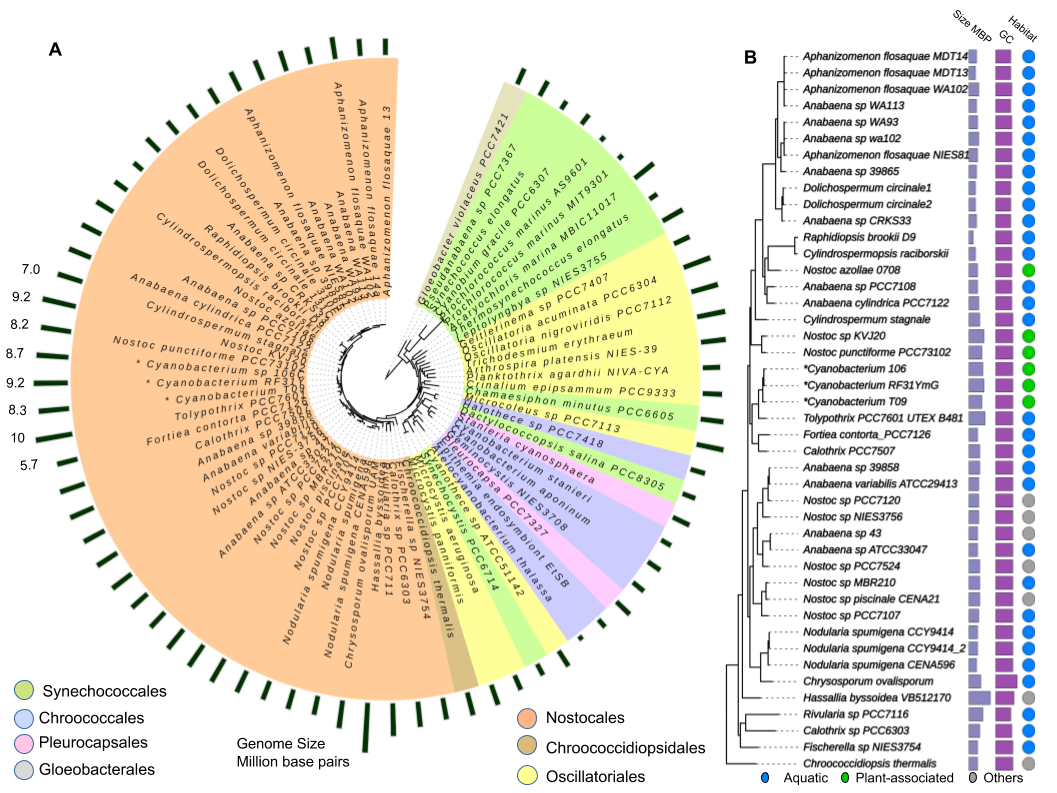
\includegraphics[angle = 0,scale = .45]{chapter1/Nostoc.png}
\caption[Arbol filogenético de $Nostoc$ construido utilizando  la selección de genes del $core~conservado$]{\footnotesize{Reconstrucción de 76 taxa provenientes de 7 órdenes de Cyanobacteria. La matriz final incluyó 45,475 aminoácidos curados de 198 familias de proteínas pertenecientes al $core~conservado$. A la derecha se muestra un zoom sobre el orden $Nostocales$. En este orden se incluyen algunas bacterias simbiontes de cícadas. Metadatos como el tamaño de genoma, contenido de GC y hábitat de origen muestran una posible tendencia de incremento de tamaño en los genomas provenientes del microbioma de plantas.}}
\label{fig:ArbolNostoc}
\end{figure}

Las Cyanobacterias son un phylum de bacterias que se han adaptado a
diversos ambientes. Aunque muchas de ellas son marinas algunas
Cyanobacterias viven como simbiontes de plantas. En particular las
cícadas han desarrollado un tipo especial de raíz donde se sabe que vive
como simbionte el género \emph{Nostoc}. La presencia de \emph{Nostoc} en
la raíz coraloide de las cícadas es fácilmente distinguible por la
formación de un anillo verde conocido como anillo cyanobacterial. En la
\autoref{fig:ArbolNostoc} se muestra la filogenia de 76 Cyanobacterias
de 7 órdenes distintos construida con 198 proteínas del core conservado
obtenidas por Orthocore. En esta reconstrucción se puede observar que
los \emph{Nostoc} asociados a plantas tienden a agruparse en la
filogenia.

\subsubsection{Identificación de genes marcadores de Clavibacter
michiganensis}\label{identificacion-de-genes-marcadores-de-clavibacter-michiganensis}

\emph{Micrococcales} es un orden de Actinobacteria que contiene a
\emph{Clavibacter}, \emph{Micrococcus} y \emph{Microbacterium}, entre
otros microorganismos. El género \emph{Clavibacter} comprende especies
que pueden causar enfermedades en diversas plantas. En particular la
especie \emph{Clavibacter michiganensis} es una bacteria causante de la
enfermedad del cáncer del tomate. \emph{Clavibacter michiganensis} ha
sido frecuentemente aislada en compañía de otros \emph{Micrococcales}
morfológicamente parecidos. La distinción entre microorganismos debida a
la comparación de la secuencia de 16s no era suficiente para distinguir
entre \emph{Micrococales} del microbioma del tomate, por lo que una
prueba de diagnóstico se hacía necesaria. Se habían utilizado como
marcadores genes como \emph{tomA}, \emph{ppaC} y \emph{celA} entre
otros, sin embargo estas elecciones en ocasiones resultaban en falsos
positivos según árboles de especies de 16s, por lo que nuevos marcadores
eran necesarios.

\begin{figure}[h!tbp]
\centering
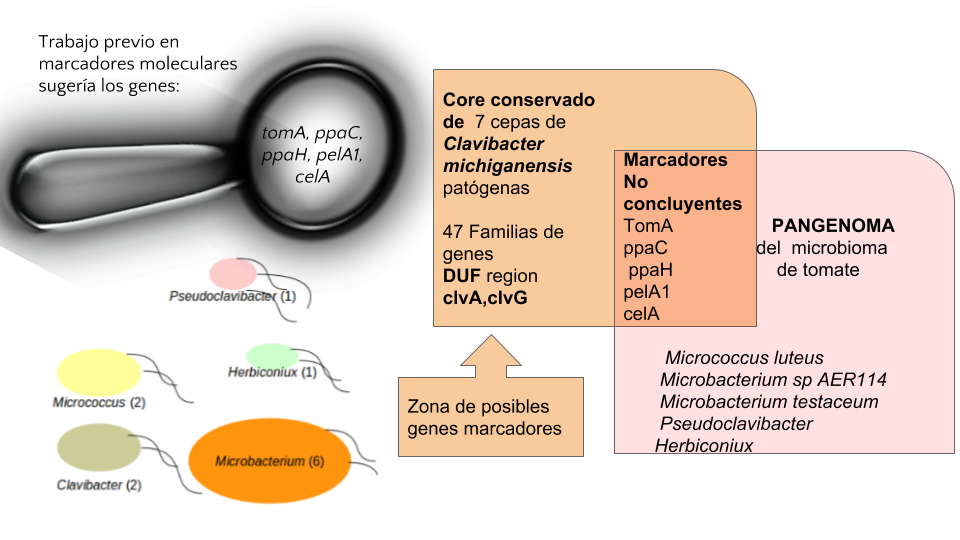
\includegraphics[angle = 0,scale = .5]{chapter1/Marcadores-Clavibacter.png}
\caption[Los genes del cluster biosintético clv son marcadores de $Clavibacter$]{\footnotesize{Los marcadores moleculares previos a este trabajo no permitían diferenciar correctamente a $Clavibacter~michiganensis$ respecto al microbioma del tomate en invernaderos mexicanos. Arriba a la izquierda se muestran los antiguos marcadores $tomA, ppaC, ppaH, pelA1, celA$. Abajo organismos pertenecientes al microbioma del tomate. Orthocore obtuvo el core conservado de siete cepas de $Cmm$ patógenas, y este core se utilizó para definir nuevos marcadores. Aunque $tomA$ pertenecía al core conservado de $Cmm$, estaba también incluido en el pangenoma del microbioma del tomate. Después de calcular la intersección core conservado de $Cmm$ y pangenoma del microbioma se obtuvieron entre las familias marcadoras genes $clv$ parte del cluster biosintético de clavidicina (michiganina).}}
\label{fig:Marcadores}
\end{figure}

Al analizar en RAST genomas de \emph{Microbacterium} y
\emph{Micrococcus} aislados de tomate se encontró que en efecto,
\emph{tomA} y los otros marcadores propuestos previamente no eran
exclusivos de \emph{Clavibacter michiganensis} ( \emph{Cmm} ). Al
utilizar Orthocore en siete genomas de \emph{Cmm} encontramos que varios
genes del cluster biosintético de michiganina (BGC0000528 en MIBiG)
codificado por los genes \emph{clvAFGLKM} pertenecían al core
conservado, pero que al agregar los genomas no Cmm del resto del
microbioma del tomate los genes \emph{clv} se pierden. El descubrimiento
de que \emph{clv} pertenecía al core de \emph{Cmm} se realizó con
secuencias de genomas muy fragmentados, en la\autoref{fig:Marcadores} se
muestran las cepas originales que fueron analizadas.

\begin{figure}[h!tbp]
\centering
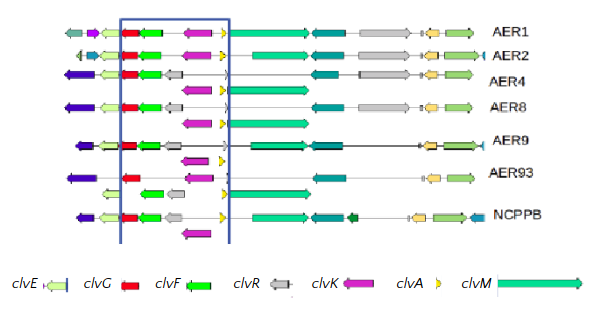
\includegraphics[angle = 0,scale = .6]{chapter1/clv.png}
\caption[ El Cluster $clv$ es un marcador de la especie $Clavibacter~Michiganesis$ en el orden $Micrococcales$.]{\footnotesize{El Cluster $clv$ es un marcador de la especie $Clavibacter~Michiganesis$ en el orden $Micrococcales$. Los genes $clvEGAM$ que son una proteína de membrana, un transportador y dos proteína de síntesis del BGC $clv$ están muy conservados en la especie $Clavibacter~Michiganensis$. $clvFRK$, es decir un transportador y el sistema de dos componentes están presentes en otros $Micrococcales$ pero con baja identidad de secuencia y nunca enel contexto del BGC de clavidicina}}
\label{fig:clv-Marcadores}
\end{figure}

Esta observación se corroboró con más genomas,
\autoref{fig:clv-Marcadores} en este caso se muestran como ejemplo 10
genomas de bacterias del microbioma del tomate, entre ellas siete
\emph{Clavibacter}, seis de tomates de invernadero y uno
\emph{Clavibacter} proveniente de tomate silvestre, \emph{Clavibacter}
RA1B que fue reportado en la tesis de maestría de Yanez. Con Orthocore
vemos que el tamaño del core decrece al ir agregando genomas de
\emph{Clavibacter} y decrece aún más rápido al agregar los genomas de
\emph{Micrococcus} y \emph{Microbacterium} La reconstrucción
filogenetica de este microbioma, ubica a \emph{Clavibacter} RA1B cerca
de los otros \emph{Cmm} pero no en un clado junto con ellos. Una
búsqueda por blast revela que los genes marcadores de \emph{Cmm}:
\emph{clvF}, \emph{clvR} son también marcadores de \emph{Clavibacter}
RA1B pero no así \emph{clvA} y \emph{clvG} que solamente están presentes
en el core de \emph{Cmm}. Sin embargo \emph{clvF} y \emph{clvR} no están
en el contexto del cluster de michiganina en RA1B y su similitud de
secuencia es menor que la que se observa entre los otros \emph{Cmm}.

De hecho al considerar más genomas dentro del microbioma del tomate, la
familia \emph{clvF} no solo no está en el core conservado de
\emph{Microbacterium} y \emph{Micrococcus}, sino que no está presente en
ningún otro genoma distinto a \emph{Clavibacter}. Con distintos niveles
de conservación de secuencia los genes \emph{clv} son un buen marcador
para distinguir \emph{Cmm} de otras especies, por esta razón estos genes
aún se encuentran en uso como genes marcadores de \emph{Cmm}. Esta misma
conclusión se reporta en el trabajo de yasuhara, su observación de que
las familias \emph{clvA, clvF} y \emph{clvG} son exclusivas de
\emph{Cmm} es independiente de la nuestra, fue hecha sin análisis
genómicos y basada en evidencia experimental
{[}@yasuhara-bell\_genes\_2014{]}. Este descubrimiento ha permitido
bajar los costos de identificación de Clavibacter, ya que ahora en lugar
de enviar a secuenciar el genoma es suficiente identificar por PCR
\emph{clvF} en conjunto con otro marcadores.

Con Orthocore además de obtener los genes marcadores podemos obtener
también la matriz del core conservado para realizar la reconstrucción
filogenética de especies cercanas de \emph{Clavibacter}
\autoref{fig:Clavibacter-EvoMining} . Debido a que es importante para
los agricultores conocer de dónde provienen las bacterias que infectan
al tomate, una de las líneas de investigación del laboratorio de
evolución de la diversidad metabólica, es la organización taxonómica de
cepas de \emph{Cmm} y de otras bacterias del microbioma de tomate. Por
este motivo se han secuenciado y mantenido como datos privados unos
doscientos genomas provenientes del microbioma del tomate. Orthocore
colabora con esta investigación proporcionando matrices multilocus que
pueden diferenciar entre cepas de \emph{Clavibacter} de la misma o de
diferente especie.

\begin{figure}[h!tbp]
\centering
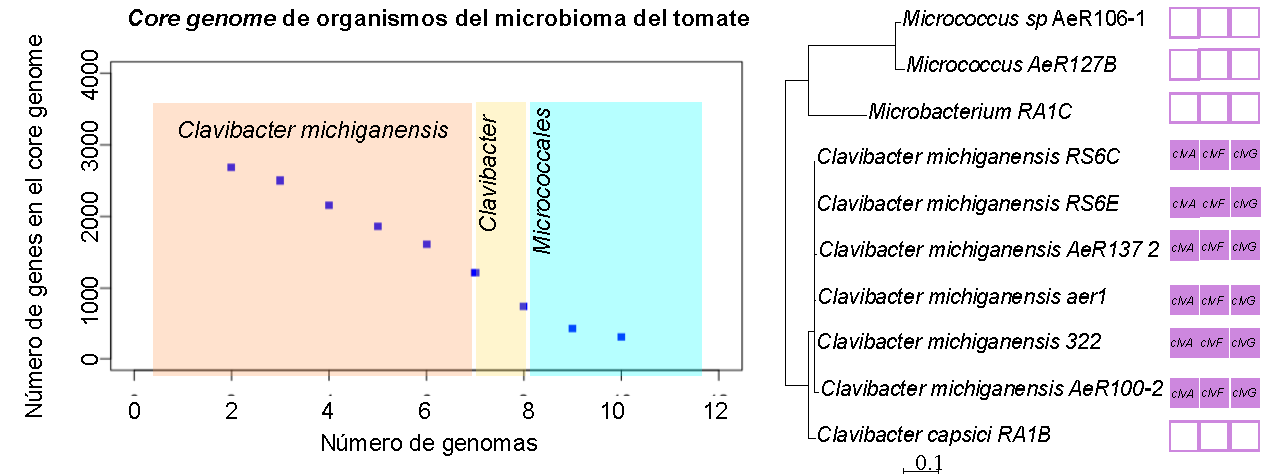
\includegraphics[angle = 0,scale = .7]{chapter1/CoreGenomeMicrobioma.pdf}
\caption[El $core~genome$ de $Micrococcales$ ayuda a identificar genes marcadores ]{\footnotesize{El $core~genome$ de $Micrococcales$ ayuda a identificar genes marcadores. El $core~genome$ de siete organismos del microbioma del tomate muestra  de }}
\label{fig:Clavibacter-EvoMining}
\end{figure}

Debido al intercambio génico por transferencia horizontal en las
bacterias, es posible que los genes marcadores actuales alguna vez
aparezcan en otros organismos. También las bacterias pierden
continuamente genes, por lo que es posible que algún gen marcador de Cmm
se pierda en una cierta cepa . Esto hace que la definición de estar
presentes en el core del grupo de interés y ausentes totalmente de cada
uno de los genomas de otro linaje ya no funcione completamente. Sin
embargo, en estas dos situaciones presentadas, ganancia de genes
marcadores de organismos externos al linaje original o pérdida de genes
marcadores en algunas cepas, se sigue cumpliendo que los ex genes
marcadores, estarán presentes en la mayoría de los organismos del linaje
de interés y ausentes de la mayoría de los organismos del linaje
externo. Por ello, se pensó que está definición de genes marcadores se
podía generalizar clasificando a grupos de genes ortólogos acorde a sus
porcentajes de ocurrencia. Esta idea se desarrolló en la herramienta
clavisual, explicada en la siguiente sección.

\subsection{Clavisual: Identificación de genes marcadores a un cierto
porcentaje de grupos
seleccionados}\label{clavisual-identificacion-de-genes-marcadores-a-un-cierto-porcentaje-de-grupos-seleccionados}

La idea de que Orthocore puede ser usado para obtener los genes
marcadores de un grupo taxonómico frente a otro fue generalizada en el
backend del software Clavisual. Ya se ha explicado previamente que el
core puede salir vacío por diversas razones, entre ellas baja calidad de
los genomas, o que éstos provengan de organismos muy divergentes,
verdaderas razones biológicas como dinámica génica o un core no
convergente. Así pues, es posible que si sólo se utiliza el core no se
obtengan marcadores. Pero el core puede relajarse de varias maneras una
de ellas es el Pseudocore, donde en lugar de multidireccional hits se
toman BBH a un genoma de referencia. Otra forma es establecer un
porcentaje de presencia /ausencia de interés.

El pseudocore consiste en \_\_\_\_\_\_\_\_ y la metodología está
depositada en github en el repositorio\_\_\_\_\_\_\_\_\_. El blast fue
optimizado cambiando hacer un blast todos contra todos por archivos
genómicos individuales genomai\_vs\_genomaj.blast que luego son
concatenandos según se necesiten.

Los porcentajes de genomas son diferentes porque al no bastar los best
bidireccional hits conservados, todo el pangenoma es decir todos los
genes contenidos en los genomas del grupo de interés necesitan ser
clasificados por familias, para de ahi obtener las familias que tienen
presencia en un porcentaje \%p y ausencia en un porcentaje a\% del grupo
externo. Estos perfiles fueron desarrollados para Clavisual
\autoref{fig:Clavisual} utilizando FasthOrtho para clasificar las
familias y de ahi obtener los grupos. Con ellos se consiguieron
marcadores para Kurtobacterium.

Finalmente Clavisual despliega un árbol realizado con el Pseudocore
respecto a un conjunto de genes de Cmm NCPP previamente seleccionados.
En este árbol clavisual permite la visualización de metadatos, como año,
género de la bacteria, estado de salud de la planta e invernadero donde
fue aislada.

\begin{figure}[h!tbp]
\centering
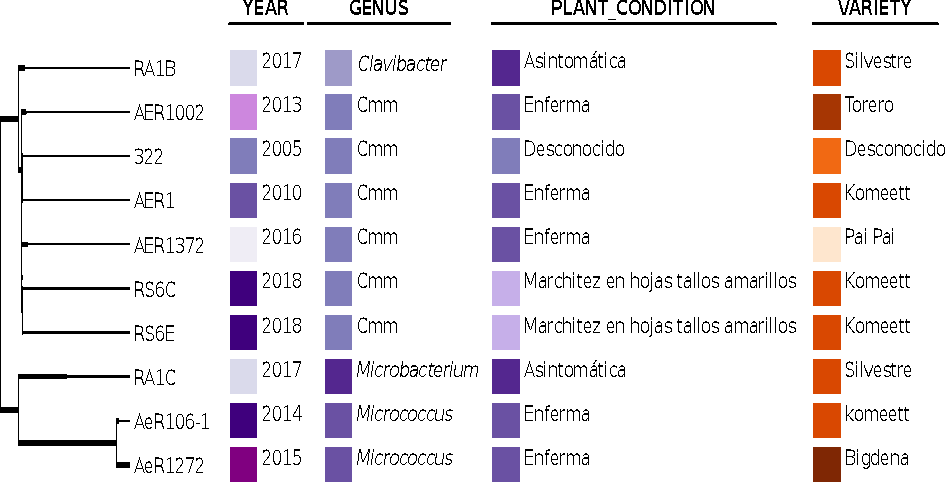
\includegraphics[angle = 0,scale = .7]{chapter1/Clavisual.pdf}
\caption[Clavisual organiza filogenéticamente cepas de $Clavibacter$ ]{\footnotesize{Aqui vemos un arbol}}
\label{fig:Clavisual}
\end{figure}

\subsubsection{El pangenoma de Clavibacter Michiganensis es
abierto}\label{el-pangenoma-de-clavibacter-michiganensis-es-abierto}

Después de desarrollar métodos de identificación de genes marcadores y
generalizarlo a obtener grupos con patrones de presencia/ausencia
definidos por el usuario, quedaba por responder la pregunta cómo es el
pangenoma de \emph{Cmm}. Algunos autores consideran que el pangenoma de
patógenos es reducido porque sus genomas suelen sufrir proceso de
reducción de tamaño débido a la pérdida de genes. Como \emph{Cmm} es un
patógeno de planta quedaba por investigar cómo es su pangenoma. ¿Es
posible saturar el contenido génico de \emph{Cmm} con sólo secuenciar
más genomas?. Aunque actualmente existen ya herramientas web para el
análisis de pangenoma, en su momento se utillizó el software bpga que se
corre desde la terminal. Para facilitar su instalación se desarrolló un
docker que se describe más tarde en este capítulo en la sección de las
descripciones técnicas. Como ejemplo de su funcionamiento, se analizó el
pangenoma de los mismos diez genomas del pangenoma del tomate utilizados
en la visualización de clavisual \autoref{fig:bpga-pangenoma} .

\begin{figure}[h!tbp]
\centering
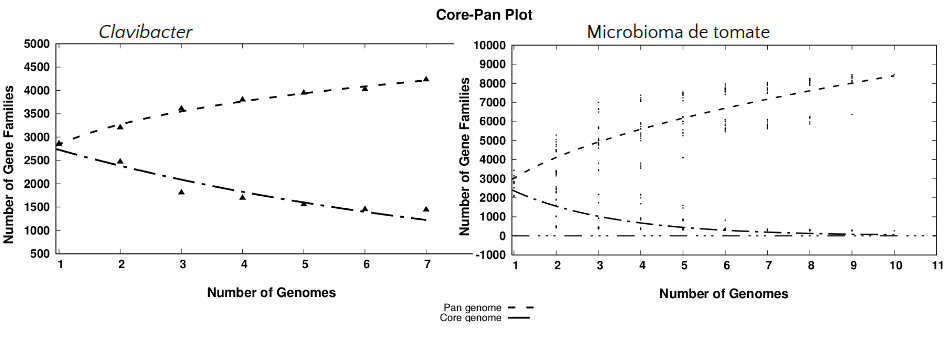
\includegraphics[angle = 0,scale = .5]{chapter1/bpga-pangenoma.png}
\caption[ X X]{\footnotesize{Pangenoma de $Clavibacter$ calculado por BPGA }}
\label{fig:bpga-pangenoma}
\end{figure}

Tomando otros siete genomas del género \emph{Clavibacter}, utilizando
OrthoVenn tenemos la misma observación, el número de familias de genes
agregadas al adicionar genomas, es después de siete genomas casi tan
grande como su core \autoref{fig:Venn-Chart}.

\begin{figure}[h!tbp]
\centering
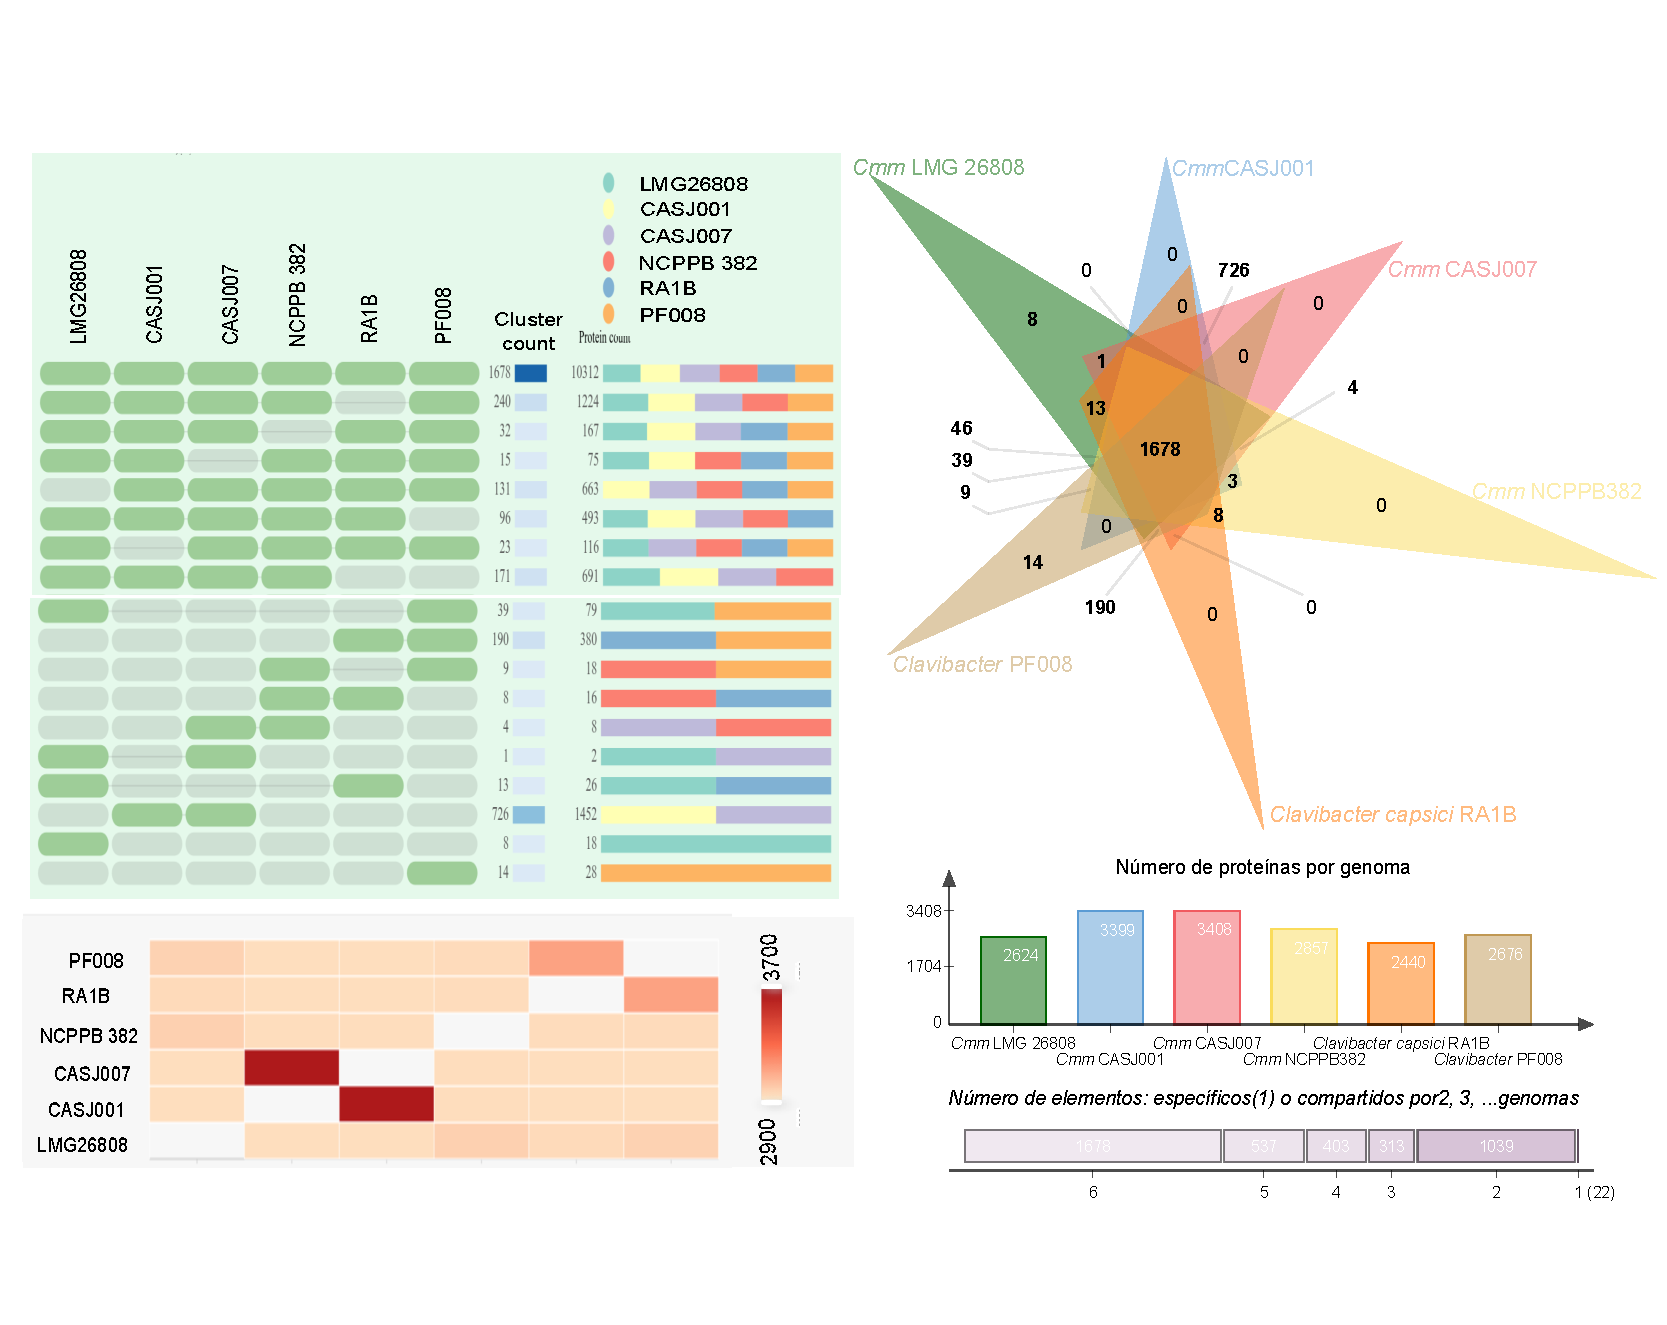
\includegraphics[angle = 0,scale = .6]{chapter1/Venn_chart.pdf}
\caption[Diagrama de Venn del pangenoma de genomas selectos del género $Clavibacter$ ]{\footnotesize{Diagrama de Venn del pangenoma de genomas selectos del género $Clavibacter$ }}
\label{fig:Venn-Chart}
\end{figure}

\subsection{Relación entre genes marcadores, Orthocores y la
promiscuidad
enzimática.}\label{relacion-entre-genes-marcadores-orthocores-y-la-promiscuidad-enzimatica.}

Finalmente, al aplicar Orthocore para detectar genes marcadores se
vuelve indirectamente reclutamientos al metabolismo especializado, cómo,
pues porque dentro de los marcadores hay productos naturales como,
PENDIENTE VER RESULTADOS RETRO-EVOMINING la clavidicina (michiganina).
Ahí vemos que clvABCDEF participan en metabolismo secundario, las
enzimas de metabolismo central de este cluster pueden presentar cierta
promiscuidad.


\end{document}
